Os efeitos dos solutos nas propriedades físicas da água podem ser vistos em algumas situações comuns e de fácil compreensão, como por exemplo, ao evitar o congelamento da água nos radiadores de carros em lugares muito frios. Os gráficos abaixo foram construídos após a avaliação da variação na temperatura de congelamento de duas soluções aquosas: uma constituída pelo soluto A e outra constituída pelo soluto B.

\begin{center}
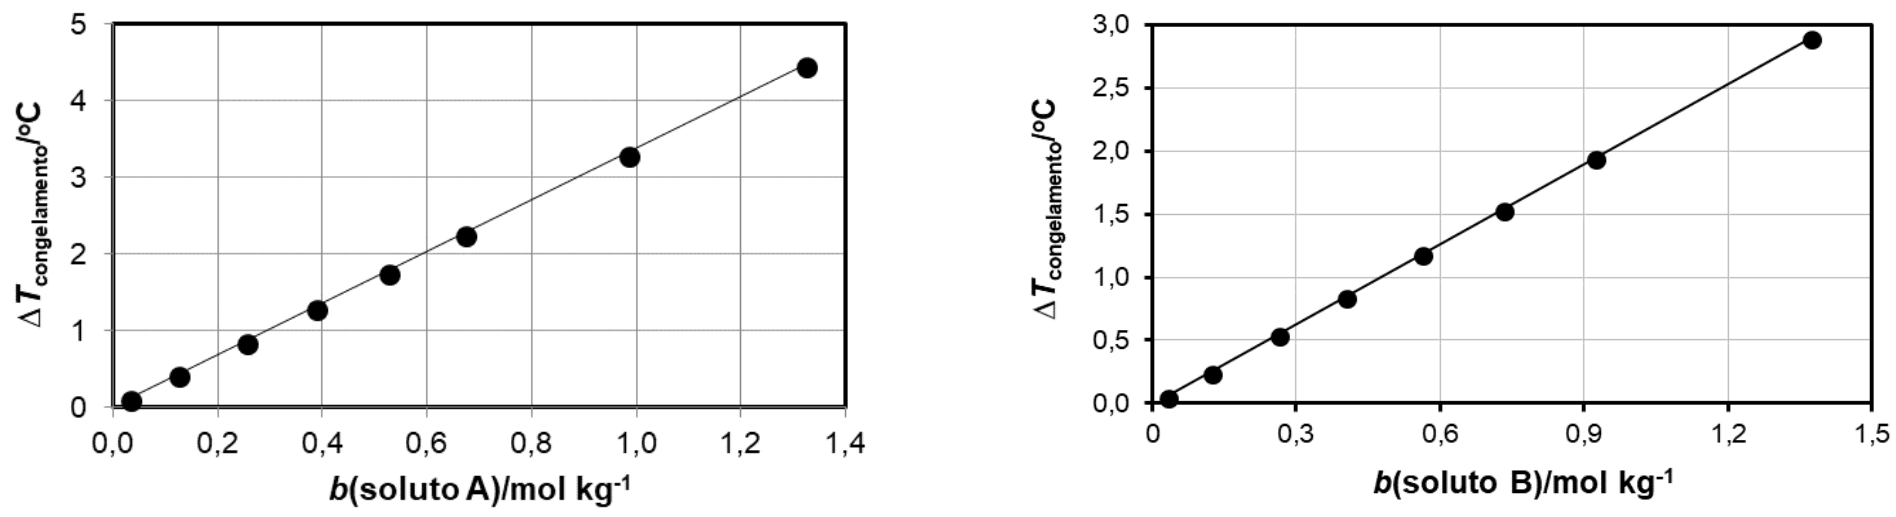
\includegraphics[width=0.8\textwidth]{figure.png}
\end{center}

Considerando as informações contidas nos gráficos pode-se afirmar que os solutos A e B eram respectivamente: 

\begin{enumerate}[label = (\alph*)]
	\item Brometo de cálcio e cloreto férrico.
	\item Cloreto de potássio e sulfato de sódio.
	\item Glicose e cloreto de sódio.
	\item Sacarose e glicose.
	\item Iodeto de potássio e sacarose.
\end{enumerate}
